\documentclass[11pt]{article}
\usepackage[letterpaper,margin=1.03in,top=0.88in,bottom=0.90in]{geometry}
\usepackage{amsmath,amssymb,amsthm,mathtools}
\usepackage{xcolor,graphicx,hyperref}
\definecolor{ink}{RGB}{26,65,83}
\hypersetup{colorlinks=true,linkcolor=ink,citecolor=ink,urlcolor=ink,pdftitle={Small-time laws for the Dirichlet Li heat kernel},pdfauthor={OpenAI}}
\newtheorem{theorem}{Theorem}[section]
\newtheorem{lemma}[theorem]{Lemma}
\newtheorem{proposition}[theorem]{Proposition}
\newtheorem{corollary}[theorem]{Corollary}
\theoremstyle{remark}\newtheorem{remark}[theorem]{Remark}
\newcommand{\R}{\mathbb R}\newcommand{\T}{\mathbb T}\newcommand{\Z}{\mathbb Z}\newcommand{\N}{\mathbb N}
\DeclareMathOperator{\dist}{dist}
\setlength{\emergencystretch}{2em}
\allowdisplaybreaks[2]
\newcommand{\pinned}[2]{\href{https://github.com/VladimirReshetnikov/ProveIt/blob/b6253012cf30c80a989c871906e097a27f23a27c/Analysis/GeneralizedRiemannHypothesis/#1}{#2}}
\title{Small-time laws for the Dirichlet Li heat kernel\\[4pt]
\large Representation counts at zero angles and a sharp law at typical points}
\author{Research note prepared for Vladimir Reshetnikov}
\date{27 November 2026}
\begin{document}
\maketitle
\begin{abstract}
The Li coefficients of a primitive Dirichlet character define a probability
density $p_t$ on the circle once its zeros are placed on the critical line.
We determine its small-time order away from the origin. At any point first
reachable as a sum of $k$ Cayley angles of zeros, a rescaled copy of the
central Cauchy profile appears. Its coefficient counts all ordered minimal
representations, including multiplicity. At every point outside the
countable union of these sumsets the density decays faster than every
power of $t$. More precisely, for almost every point and for the minimum
over the whole circle, its negative logarithm is asymptotic to
$\log(1/t)\log\log(1/t)/\log 2$. The same constant governs the least number
of zero angles needed to approximate a typical point. A residual set has
every intermediate normalized decay rate as a subsequential limit.
For $0<h\le1/\log2$, the set on which the lower normalized decay rate
equals $h$ has Hausdorff dimension $(e^{1/h}-1)^{-1}$. The zero-rate
level is residual and has dimension zero. The construction retains the
sign of each ordinate for complex characters.
\end{abstract}
\section{The observation and what it determines}
Fix a primitive Dirichlet character $\chi$ of conductor $q$, allowing $q=1$
for the Riemann zeta function. Use the Dirichlet zero-line theorem
of the supplied Lean development. Count each nontrivial zero
$\rho=1/2+i\gamma$ with its multiplicity. Its Cayley phase is
\[
 z_\rho=1-1/\rho=e^{i\theta_\gamma},\qquad
 \theta_\gamma=2\arctan(1/(2\gamma))\quad(\gamma\ne0),\qquad \theta_0=\pi.
\]
Use arc length on $\T=\R/(2\pi\Z)$, so a probability density integrates to
one on $[-\pi,\pi]$. The observations are the Li coefficients in the
following convention, and the resulting density:
\begin{equation}\label{eq:observation}
 \lambda(n)=\lim_{T\to\infty}\sum_{|\gamma|\le T}(1-z_\rho^n),
 \qquad p_t(x)=\frac1{2\pi}\sum_{n\in\Z}e^{-t\lambda(n)}e^{-inx}.
\end{equation}
In particular $\lambda(0)=0$ and $\lambda(-n)=\overline{\lambda(n)}$.
We prove convergence and positivity below. The \emph{jump order} of a point is the
least $k$ for which $e^{ix}$ is a product of $k$ zero phases, with
repetitions allowed. The empty product has order zero.
For a point of finite jump order $k$ let $M_k(x)$ be the number of ordered
representations of length $k$, with each choice weighted by the
multiplicity of each chosen zero. The same occurrence can be used more
than once.

Write $L=\log(1/t)$, and put
\begin{equation}\label{eq:scale}
 \kappa=\gamma_{\mathrm E}+\log(q/(2\pi))-1,\quad
 w=W_0(2e^\kappa/t),\qquad a=a(t)=tw/2\sim tL/2 .
\end{equation}
Here $W_0$ is the inverse of $w\mapsto we^w$ on the positive axis.
The following statements describe the different scales on which the
same density can be observed.
\begin{theorem}\label{thm:summary}
For each fixed primitive $\chi$ the following hold.
\begin{enumerate}
\item If $x$ has finite jump order $k$, locally uniformly in $z\in\R$, with
all fixed orders of differentiation,
\[
 \frac{a}{t^k}p_t(x+az)\longrightarrow
 \frac{M_k(x)}{k!}\,\frac1{\pi(1+z^2)}.
\]
In fact $k!p_t(x)/(t^k p_t(0))=M_k(x)+O_x(t)$.
At every point of infinite jump order, $p_t(x)=O_{x,H}(t^H)$ for every $H>0$.
\item For arc-length almost every $x$,
\[
 \frac{-\log p_t(x)}{L\log L}\longrightarrow\frac1{\log2}.
\]
The same limit holds with $p_t(x)$ replaced by $\min_{u\in\T}p_t(u)$.
Approximating almost every $x$ to within $h$ requires asymptotically
$\log\log(1/h)/\log 2$ angles, and this many up to an additive constant
suffices for every $x$.
\item If $F(x)=\liminf_{t\downarrow0}-\log p_t(x)/(L\log L)$, then
\[
 \dim_{\rm H}\{x:F(x)=h\}=\frac{1}{e^{1/h}-1}
 \qquad (0<h\le1/\log2).
\]
The set $F=0$ is a dense $G_\delta$ of dimension zero.
On a dense $G_\delta$ subset of $\T$ the set of subsequential limits
of $-\log p_t(x)/(L\log L)$ is the whole interval $[0,1/\log 2]$.
\end{enumerate}
\end{theorem}
In particular the multiplicity of a zero at $1/2+i\gamma$ equals the limit
of $p_t(\theta_\gamma)/(t p_t(0))$. The sign of the ordinate is retained even
when $\chi$ is nonreal. Higher orders read multiplicative relations among
the $z_\rho$. No separation bound for the zeros, simplicity conjecture or
independence of their angles enters the formulas. Section~\ref{sec:zetapeaks}
gives a pair of adjacent two-jump peaks for which the limiting heights
are in the ratio $1:2$.

\paragraph{Sources and scope.}
The vendored \pinned{vendor/grh-lean/grh/src/Main.lean}{\texttt{Main.lean}}
exports \texttt{LFunction\_eq\_zero\_re}, with the proposition specified in
\pinned{vendor/grh-lean/grh/src/Statements.lean}{\texttt{Statements.lean}}.
It quantifies over all characters of positive modulus and all zeros in the
open critical strip. The upstream
\pinned{vendor/grh-lean/grh/src/New/Reduction/OneSidedBound.lean}{one-sided estimate}
bounds a smoothed prime remainder and feeds a criterion for nonvanishing
to the right of $1/2$. The
\pinned{vendor/grh-lean/grh/src/New/Main.lean}{functional-equation step}
applies that bound to both $(\chi,s)$ and $(\chi^{-1},1-s)$.
Geometrically its conclusion is $|1-1/\rho|=1$, the condition that makes
all jumps in \eqref{eq:observation} rotations. The vendored tree is the readable edition of
\href{https://github.com/lsernau/grh-lean/tree/72fead102f663d5c7a407964a13dc0cf9d977207/grh}{\texttt{lsernau/grh-lean} at \texttt{72fead102f66}}.
Its published checker results and pinned software are documented in the
\pinned{vendor/grh-lean/grh/README.md}{vendor README}.
We inspected the declarations and source provenance.
We did not rerun its Lean kernel or formalize the present proofs.
The merged article's
\pinned{Article/sections/src.tex}{source section} sets out the scope of that input.
Its \pinned{Article/sections/li.tex}{Li section} constructs the symmetrized
jump process and derives its expansion at the origin, including the Cauchy
profile. Its \pinned{Article/sections/rec.tex}{reconstruction section}
uses signed complex Li data. The off-origin representation law, the metric
constant and the dimension spectrum are the extensions proved here.
The matching constant concerns jump sizes near zero and their abundance.
The zero-line theorem enters to identify those jumps with the phases in
the actual arithmetic Li coefficients. One may construct a process from
ordinates alone without that identification.

\paragraph{Earlier results.}
Nakamura and Suzuki~\cite{nakamura} associated a compound Poisson law
with zeta zeros using inverse-square weights on the ordinates.
Lagarias obtained the complex Li asymptotic and one-sided zero counts
used here~\cite{lagarias}. Picard studied small-time densities at points
reachable in finitely many jumps and at limits of such points. His
discrete examples relate the polynomial order to least jump number, and
his dyadic model exhibits a different almost-everywhere logarithmic rate
\cite{picard1,picard2}. In particular, Picard's dyadic Example 6.4
has a squared-logarithm scale. Wu~\cite{wu} studied exceptional growth in
the denominators of the canonical Sylvester expansion. Here the approximation
is optimized over all finite sums of the allowed angles. The claims here concern the actual coefficient
and local profile at each sum, the exact $L\log L$ scale and its Hausdorff level sets for the
Cayley-angle sequence. The comparison with these sources and the
requested repository establishes the scope of the contribution;
historical priority has not been independently established.

\section{The signed process and its central profile}\label{sec:central}
The one-sided zero counts, for either sign, satisfy
\begin{equation}\label{eq:zero-count}
 N_\pm(T)=\frac{T}{2\pi}\log\frac{qT}{2\pi e}+O_\chi(\log(2+T))
\end{equation}
by~\cite[Theorem 2.1(4)]{lagarias}; treatment of a central zero changes only
a bounded term. In particular, $\nu=\sum_\gamma\delta_{\theta_\gamma}$
on the principal real interval $(-\pi,\pi]$ has
$V=\int y^2\nu(dy)<\infty$ by partial summation. The signed principal
value $b_0=\lim_{T\to\infty}\sum_{|\gamma|\le T}\theta_\gamma$ exists.
Indeed, $D(T)=N_+(T)-N_-(T)=O_\chi(\log(2+T))$ and
$\theta'(v)=-(v^2+1/4)^{-1}$ on the positive axis. Partial summation gives
a convergent tail. It follows that
\[
 \Psi(u)=\int(1-e^{iuy}+iuy)\,\nu(dy)-iu b_0
\]
is the characteristic exponent of a real L\'evy process $X_t$, with
$\mathbb E e^{iuX_t}=e^{-t\Psi(u)}$. The expression is exactly the
symmetric-height sum of $1-e^{iu\theta_\gamma}$. Reduction of $X_t$ modulo
$2\pi$ gives \eqref{eq:observation} because $\Psi(n)=\lambda(n)$.
Finite sets of jumps can always be split off as ordinary uncompensated
compound Poisson processes; the remaining drift is fixed by this convention.

\begin{lemma}[Central scale]\label{lem:core}
For any fixed nonnegative integer $r$,
\begin{align}
 a p_t(az)&\longrightarrow Q_0(z)=\frac{1}{\pi(1+z^2)}
       &&\text{in } C^r\text{ on compact intervals},\label{eq:core}\\
 a^{r+1}\sum_{n\in\Z}|n|^r e^{-t\Re\lambda(n)}&=O_{\chi,r}(1).
       \label{eq:deriv}
\end{align}
For $r=0$ take the zeroth power to equal one at $n=0$.
Moreover the oriented kernel has the same central expansion to every order
in $1/w$ as the symmetrized kernel of the merged article.
\end{lemma}
\begin{proof}
Lagarias's complex Li asymptotic, or the symbol calculation in the
Li section of the article together with the following imaginary-part
estimate, gives for integers $n\ge2$
\[
 \lambda(n)=\tfrac12 n(\log n+\kappa)+O_\chi(\sqrt n\log(2+n)).
\]
For the imaginary part, ordinates of magnitude at most $\sqrt n$ cost
$O(\sqrt n\log n)$ trivially. The remaining signed sine sum is an integral
against $dD(v)$. Integration by parts bounds its absolute value by
$O(\log n+n\int_{\sqrt n}^\infty \log(2+v)v^{-2}dv)$, as required.
In particular $e^{-t\lambda(n)}$ decays faster than every exponential in
$|n|$ for each $t>0$. Fourier inversion gives an entire periodic density.

For $s=a|n|$ in a fixed compact subinterval of $(0,\infty)$ the real
main exponent is $s+s\log s/w$ and the complex error is
$O_\chi(t\sqrt{|n|}\log(2+|n|))=o(1)$ uniformly there. For $s\ge1$
the modulus of the multiplier is at most $Ce^{-cs}$ for all small $t$,
as $\log(1/a)=w-\kappa$. For $s\le1$ it is at most one. The Riemann
sums of mesh $a$ give \eqref{eq:deriv} and the inverse Fourier transform
of $e^{-|s|}$ gives \eqref{eq:core}, with polynomial weights for derivatives.
For the all-orders assertion compare with the symmetrized multiplier
$e^{-t\Re\lambda(n)}$. The scaled sum of the absolute differences, weighted
by $|an|^r$, is $O_r(\sqrt a)$. The range $a|n|\le\sqrt a$ costs
$O(\sqrt a)$. On the rest use
$|e^{-it\Im\lambda(n)}-1|\le t|\Im\lambda(n)|$, the estimate above, and
$e^{-t\Re\lambda(n)}\le C e^{-c a|n|}$ (enlarging $C$ for $a|n|\le1$).
Since $t=2a/w$, summation costs $O(\sqrt a)$ there as well.
The article proves the all-orders expansion for the real-part multiplier
on compact rescaled intervals. Finally $\sqrt a=o(w^{-j})$ for every $j$.
\end{proof}

\section{Exact profiles at finite sums}\label{sec:finite}
Write $S_0=\{0\}$ and let $S_k$ be the $k$-fold sum of
$\{0\}\cup\operatorname{supp}_{\rm at}\nu$ in $\T$, where
$\operatorname{supp}_{\rm at}$ means the points of positive atomic mass.
The only accumulation point of the individual angles is zero, so each
$S_k$ is compact and countable. Every point of $S_k\setminus S_{k-1}$
is isolated in $S_k$. Otherwise take a sequence of distinct sums tending
to it, pass to coordinatewise convergent subsequences, and use compactness.
A limit tuple with a zero coordinate gives a point of $S_{k-1}$. If all
coordinates are nonzero, they are isolated and the tuples are eventually
constant. The same argument shows the minimal representations are finite.
Moreover every summand in a representation of $x$ of length $k$ has
distance at least $\dist(x,S_{k-1})$ from zero.

\begin{proposition}[Relative profile and multiplicity]\label{prop:profile}
For $x\in S_k\setminus S_{k-1}$, $k\ge1$, every fixed $R,r$ and small $t$,
\begin{equation}\label{eq:relative}
 \left\|a p_t(x+a\,\cdot)-
  \frac{M_k(x)}{k!}\,t^k a p_t(a\,\cdot)\right\|_{C^r([-R,R])}
     =O_{x,k,R,r}(t^{k+1}).
\end{equation}
If $x\notin\bigcup_j S_j$, the left-hand rescaled density alone
is $O_{x,H,R,r}(t^H)$ for every $H>0$.
\end{proposition}
\begin{proof}
We give the truncation details since the jump measure is atomic and has
infinite mass near zero. For fixed $\epsilon>0$, split off the finite
measure $\mu=\nu|_{|y|>\epsilon}$, of mass $\Lambda$. Let $g_t$ be the
circle density of the remaining process. In Fourier inversion its
multipliers differ from the original ones by the factor
$\exp(t\int(1-e^{iny})\mu(dy))$, of modulus at most $e^{2t\Lambda}$.
Thus \eqref{eq:deriv} holds for $g_t$ as well. In addition
\begin{equation}\label{eq:finite-removal}
 \|a(g_t-p_t)(a\,\cdot)\|_{C^r(\R)}=O_{r,\epsilon}(t).
\end{equation}
For fixed $d,H>0$ the cutoff $\epsilon$ can be chosen so small that,
uniformly in $\dist(y,0)\ge d$,
\begin{equation}\label{eq:tail}
 \|a g_t(y+a\,\cdot)\|_{C^r([-R,R])}=O(t^H).
\end{equation}
To verify this, the real lift of the remainder has drift
$b_\epsilon=b_0-\int y\mu(dy)$ in the full linear compensation convention.
For $h=L/(2\epsilon)$ its log moment generating function at either sign
of $h$ is bounded above by
$t|h b_\epsilon|+C t h^2 e^{h\epsilon}V=o(1)$.
Exponential Markov bounds the mass at circular distance at least $d/2$
by $O(t^{d/(4\epsilon)})$. For $G(z)=a g_t(y+az)$ this bounds its
integral on $[-R-1,R+1]$, where the coordinate map is injective for small
$t$. All derivatives of $G$ are uniformly bounded by \eqref{eq:deriv}.
Convolve $G$ locally with a smooth unit-mass mollifier of width $h_1=t^H$.
On $[-R,R]$ its $r$th derivative differs from that of $G$ by $O(h_1)$;
the convolved derivative is
$O(h_1^{-r-1}t^{d/(4\epsilon)})$. Choosing $d/(4\epsilon)>H(r+2)$
proves \eqref{eq:tail} for all orders up to $r$.

Choose $d>0$ smaller than the distance from $x$ to $S_k\setminus\{x\}$.
Take $\epsilon$ small enough for \eqref{eq:tail} with $H=k+1$, and
smaller than $\dist(x,S_{k-1})$. Expand the law of the removed part:
\[
 p_t=e^{-t\Lambda}\sum_{j\ge0}\frac{t^j}{j!}\,g_t*\mu^{*j}.
\]
Orders $j>k$ in the rescaled $C^r$ norm cost $O(t^{k+1})$ by
\eqref{eq:deriv}. Orders $j\le k$ away from the atom at $x$ have the
same bound by \eqref{eq:tail}. At $x$ there is precisely the atom of
$\mu^{*k}$ of mass $M_k(x)$. Using $e^{-t\Lambda}=1+O(t)$ and
\eqref{eq:finite-removal} proves \eqref{eq:relative}. For a point outside
the union, choose any fixed $k>H$, use the positive distance to the
whole of $S_k$, and run the same estimate with no surviving atom.
Since $a\asymp tL$, rescaling back costs at most one extra power of $1/t$
for the density itself. This proves the assertion about $p_t(x)$.
\end{proof}
Combining \eqref{eq:relative} with Lemma~\ref{lem:core} gives the full
central logarithmic expansion, multiplied by $M_k(x)/k!$, at each minimal
sum. Normalization by the measured central height cancels all its
logarithmic corrections and gives the $O(t)$ integer readout in
Theorem~\ref{thm:summary}. Fixed-order readings require only finitely many
Li coefficients at each $t$. For any $D>2(k+1)$ truncate
\eqref{eq:observation} at $|n|\le D/t$. For every $c<1/2$ and large $n$,
$\Re\lambda(n)\ge c n\log n$. The discarded sum, multiplied by $a$, is
$O(a\,e^{-tcN\log N}/(1-e^{-tc\log N}))=O(t^{cD})$ for
$N=\lceil D/t\rceil$. Choose $cD>k+1$. The truncation preserves the
$O(t)$ readout at a specified finite-order point. This is a pointwise
asymptotic statement; a universal finite threshold for rounding would
require quantitative bounds on distances to competing sums.

\section{The density at a typical point}
\label{sec:metric}

Let $d_{\mathbb T}$ be arc-length distance on $\mathbb T=\mathbb R/(2\pi\mathbb Z)$.
Write $S$ for the oriented Cayley angles that occur, together with $0$, and $S_m$ for all sums
of at most $m$ angles modulo $2\pi$, with repetitions allowed. Define
\[
  D_m(x)=d_{\mathbb T}(x,S_m),\qquad
  J_{\varepsilon}(x)=\min\{m\ge0:D_m(x)\le\varepsilon\}.
\]
Throughout this section all logarithms are natural, $L=\log(1/t)$, $a=a(t)$
is the central length scale, and $p_t$ is the circle density with respect to
arc length. Constants may depend on the fixed zero multiset.

\begin{theorem}[Metric approximation and heat decay]\label{thm:metricdecay}
For Lebesgue-almost every $x$ on the circle,
\[
 \lim_{\varepsilon\downarrow0}
 \frac{J_{\varepsilon}(x)}{\log\log(1/\varepsilon)}
   =\frac1{\log 2},\qquad
 \lim_{t\downarrow0}\frac{-\log p_t(x)}{L\log L}
   =\frac1{\log 2}.
\]
Moreover,
\[
  \lim_{t\downarrow0}\frac{-\log\min_{x\in\mathbb T}p_t(x)}
                                  {L\log L}=\frac1{\log 2}.
\]
\end{theorem}

\paragraph{Approximation from above.}
For each sign separately the number $N_\pm(T)$ of ordinates of that sign
and magnitude at most $T$ has the form $c_1T\log T+c_2T+O(\log T)$,
with $c_1>0$. Hence for one fixed $H>0$ every sufficiently high interval
$(T,T+H]$ contains an absolute ordinate of each sign. The change of the main
term is $c_1H\log T+O_H(1)$, while the two remainder terms cost at most
$(2C+o(1))\log T$ for a fixed $C$. The map
$u\mapsto 2\arctan(1/(2u))$ has derivative $-1/(u^2+1/4)$.
At every sufficiently small $r>0$ and for either specified sign, there is
a jump of that sign with magnitude $b$ satisfying
$0\le r-b\le C_0 r^2$. Take $T=\tfrac12\cot(r/2)$ and an ordinate of the
specified sign in the indicated range of magnitudes.

To approximate any $x$, represent it in $[-\pi,\pi]$. Subtract a bounded
number of copies of a fixed jump of the sign of $x$, chosen so small in
each direction that its magnitude $b_*$ is in the preceding range and
$C_0b_*<1/2$. The remaining magnitude is less than $b_*$.
The bound on this preliminary number is uniform in $x$. Subsequently,
choosing a jump with the sign of the current residual gives
$r_{i+1}\le C_0 r_i^2$. Hence $C_0r_i\le2^{-2^i}$. In particular,
\begin{equation}\label{eq:metricgreedy}
 \sup_x J_{\varepsilon}(x)\le
       \frac{\log\log(1/\varepsilon)}{\log2}+O(1).
\end{equation}

\paragraph{Metric lower bound for the number of jumps.}
List the distinct absolute jump magnitudes in nonincreasing order as
$b_1,b_2,\ldots$. The number of magnitudes at least $u$ is
$O(u^{-1}\log(2/u))$ for small $u$, by the same zero count.
Consequently for every $s>1$ there is a $C_s$ such that $b_j\le C_sj^{-1/s}$.

Fix $p>1$ and $0<\eta<1/(2\zeta(p))$. For almost every $x$ there is
$c_x\in(0,1)$ such that, simultaneously for $k\ge0$, signs $e_i=\pm1$
and positive indices $j_i$,
\begin{equation}\label{eq:metricBC}
 d_{\mathbb T}\left(x,\sum_{i=1}^k e_i b_{j_i}\right)
       \ge c_x\eta^k\prod_{i=1}^k j_i^{-p}.
\end{equation}
Indeed the arcs about all ordered signed tuples with radii
$\eta^k\prod j_i^{-p}$ have summed lengths bounded by
$2\sum_{k\ge0}(2\eta\zeta(p))^k$. Borel--Cantelli leaves only finitely
many exceptional tuples for almost every $x$. Excluding their countably many
possible centres, decreasing $c_x$ handles those finitely many tuples as well.
Allowing both signs of each magnitude only enlarges the comparison set.

For a tuple of length $n\le m$, $m\ge1$, order its magnitudes decreasingly.
Let $r_k$ be the distance of $x$ from the sum of its first $k$ signed
magnitudes, $d=r_n$, and $B_k=\sum_{i\le k}\log j_i$.
Stop at the first $k$ with $r_k\le2d$. Before this stopping index,
$r_k\le d+m b_{j_{k+1}}$, and
$b_{j_{k+1}}>r_k/(2m)$. The magnitude bound and
\eqref{eq:metricBC} give
\[
 B_{k+1}\le(1+sp)B_k+
    s\bigl(\log(2m C_s/c_x)+k\log(1/\eta)\bigr).
\]
Increasing $C_s$ if necessary, geometric summation from $B_0=0$ yields
$B_k\le C_{x,s,p}(1+sp)^k\log(2m)$ up to and including the stopping
index, since $\sum_{j\ge0}(1+j)(1+sp)^{-j}<\infty$.
At that index $d\ge r_k/2$, so for all $m\ge1$
\begin{equation}\label{eq:metricseparation}
 D_m(x)\ge \exp\{-C_{x,s,p}'(1+sp)^m\log(2m)\}.
\end{equation}
Intersect the full-measure sets for rational $p,s>1$. For any
$0<c<1/\log2$ take $s,p$ near enough to one that $c\log(1+sp)<1$.
With $U=\log(1/\varepsilon)$ and $m=\lfloor c\log U\rfloor$, the exponent
on the right of \eqref{eq:metricseparation} is $o(U)$.
Thus $J_{\varepsilon}(x)>m$ for every sufficiently small $\varepsilon$.
Together with \eqref{eq:metricgreedy}, this proves the first limit.

\paragraph{A lower bound for the density, uniform on the circle.}
Use \eqref{eq:metricgreedy} to choose $k\le (\log L)/\log2+O(1)$ signed
jumps with sum $z$ satisfying $d_{\mathbb T}(x,z)\le a$.
Here $a\asymp t\log(1/t)$. Remove unit mass from each distinct circle atom
on the list. Every such atom has multiplicity at least one. The resulting
finite measure $\mu$ has mass at most $k$. Write $q_t$ for the density left
after removing its independent uncompensated compound Poisson process.
The Fourier multiplier for this removal is
$\exp\{t\int(1-e^{iny})\mu(dy)\}$, up to the choice of Fourier sign.
Its difference from $1$ has modulus at most $e^{2tk}-1$. The central Fourier
bound gives $\sum_{n\in\mathbb Z}|\mathbb E e^{inX_t}|=O(1/a)$, whence
\[
  \|q_t-p_t\|_\infty\le C(e^{2tk}-1)/a.
\]
The central Cauchy limit \eqref{eq:core} gives
$\inf_{d_{\mathbb T}(u,0)\le a} a p_t(u)\ge c_0>0$ for small $t$.
Thus $q_t(x-z)\ge c_0/(2a)$ uniformly. The probability of exactly the
prescribed multiplicities in the removed process is at least
$e^{-tk}t^k/k!$. Independence yields the uniform bound
\begin{equation}\label{eq:metriclower}
  p_t(x)\ge\frac{c_0}{2a}
      \exp\left(-\frac{L\log L}{\log2}-O(L)\right).
\end{equation}

\paragraph{Upper bound at almost every point.}
Fix an $x$ satisfying \eqref{eq:metricseparation} for all rational
$p,s>1$. For $c<1/\log2$, $c>0$, choose $p,s$ with
$c\log(1+sp)<1$ and pick exponents
$c\log(1+sp)<\beta<\beta'<1$. For every sufficiently small $t$ use
\[
 m=\lfloor c\log L\rfloor,\qquad
 d=\exp(-L^\beta),\qquad b=\exp(-L^{\beta'}).
\]
Then $D_m(x)\ge d$. Split the jump measure by size at $b$.
The larger jumps are compound Poisson with intensity
$\lambda\le V/b^2$, where $V=\int y^2\nu(dy)<\infty$ in principal-angle
coordinates. In particular $t\lambda\le\exp(-L+O(L^{\beta'}))$.
Let $q_v$ denote the circle density left after removing those uncompensated
Poisson jumps, and $Y_v$ its real-valued lift with the inherited drift.
For $v=t$ and $t/2$, the modulus of each Fourier multiplier is at most
$e^{2v\lambda}$ times the corresponding full multiplier modulus, giving $\|q_v\|_\infty=O(1/a)$ since $a(t/2)\asymp a(t)$.

Write $d_0$ for the fixed real drift of the full lift in the convention
that compensates all jumps (all jump sizes have magnitude at most $\pi$).
The inherited drift in this convention is
$d_b=d_0-\int_{|y|> b} y\nu(dy)$, so $|d_b|\le|d_0|+V/b$.
For the lift,
\[
 \log\mathbb E e^{\pm Y_{t/2}/b}
 =\frac t2\left(\frac{\pm d_b}{b}
   +\int_{|y|\le b}(e^{\pm y/b}-1\mp y/b)\nu(dy)\right)
 \le C t\bigl(|d_0|/b+ V/b^2\bigr)=o(1).
\]
If $d_{\mathbb T}(u,0)\ge d$, either $v$ or $u-v$ has distance at least
$d/2$ from $0$. Splitting the convolution $q_t=q_{t/2}*q_{t/2}$ and applying
the exponential Markov inequality on the line proves
\begin{equation}\label{eq:metrictrunc}
 \sup_{d_{\mathbb T}(u,0)\ge d}q_t(u)
 \le 2\|q_{t/2}\|_\infty\Pr\{|Y_{t/2}|\ge d/2\}
 \le \frac{C}{a}\exp\left(-\frac{d}{2b}+o(1)\right).
\end{equation}
On the event of at most $m$ large jumps their sum belongs to $S_m$, so
\eqref{eq:metrictrunc} applies at the residual. On the complementary
event bound the density by $C/a$. For $N$ Poisson with mean $t\lambda$,
the factorial moment bound is
$\Pr\{N\ge m+1\}\le(t\lambda)^{m+1}/(m+1)!$.
It follows that
\[
 p_t(x)\le\frac C a\left[
 \exp\left(-\tfrac12 e^{L^{\beta'}-L^\beta}+o(1)\right)
 +\exp\left(-(m+1)\bigl(L-O(L^{\beta'})\bigr)\right)\right].
\]
Since $\log(1/a)=O(L)$, this implies
$\liminf_{t\downarrow0}(-\log p_t(x))/(L\log L)\ge c$.
Let $c\uparrow1/\log2$ and use \eqref{eq:metriclower}. The estimates hold
throughout a real interval of sufficiently small times for each $c$.
Finally, the uniform bound \eqref{eq:metriclower} and evaluation at any
single point satisfying the almost-everywhere limit give the claimed
minimum law.

\begin{corollary}[Typical points in the sense of Baire category]
Set $R_t(x)=-\log p_t(x)/(L\log L)$ for sufficiently small $t$. There is a
dense $G_\delta$ set of points outside every $S_m$ on which
\[
 \liminf_{t\downarrow0}R_t(x)=0,\qquad
 \limsup_{t\downarrow0}R_t(x)=1/\log 2.
\]
\end{corollary}

\begin{proof}
The union $\bigcup_m S_m$ is countable and dense by
\eqref{eq:metricgreedy}. At any of its points $z$, fixing one representation
by $k$ jumps in the argument of \eqref{eq:metriclower} gives
$p_t(z)\gg_z t^k/a$ and hence $R_t(z)\to0$.
The points of Theorem~\ref{thm:metricdecay} with limit $1/\log 2$
also form a dense set, by full Lebesgue measure. For integers $j\ge1$ and
$N\ge3$, each of the two open sets
\[
 \bigcup_{n\ge N}\{x:R_{e^{-n}}(x)<1/j\},\qquad
 \bigcup_{n\ge N}\{x:R_{e^{-n}}(x)>1/\log2-1/j\}
\]
contains the corresponding dense set. Positivity and continuity of the density
for all sufficiently small times follow from \eqref{eq:metriclower} and
Fourier inversion (one may increase $N$ throughout). Intersect all these
open sets and exclude the countable set of finite sums. The result is a
dense $G_\delta$ set by Baire's theorem. The uniform bounds
$p_t(x)\ll1/a$ and \eqref{eq:metriclower} give the two opposite inequalities
for the limits over all real $t\downarrow0$.
\end{proof}
For small positive times $R_t(x)$ is continuous in $t$ by locally uniform
Fourier convergence. The preceding corollary and the intermediate value theorem
give every subsequential limit between its two endpoints.
\section{Hausdorff dimension of the exceptional decay rates}
\label{sec:dimension}
Define $F(x)$ everywhere and $\omega(x)$ outside the countable union of the finite sumsets by
\[
 \omega(x)=\limsup_{m\to\infty}
      \frac{\log\log(1/D_m(x))}{m},\qquad
 F(x)=\liminf_{t\downarrow0}\frac{-\log p_t(x)}{L\log L}.
\]
Set $\omega(x)=\infty$ at a finite sum, including the origin. Greedy
approximation gives $\omega(x)\ge\log2$ everywhere.

\begin{theorem}[Exceptional decay rates]\label{thm:dimension}
For every $x$ one has $F(x)=1/\omega(x)$, with $1/\infty=0$.
The level set $\{x:F(x)=0\}$ is a dense $G_\delta$ of Hausdorff dimension zero.
For each $0<h\le 1/\log2$,
\[
 \dim_{\rm H}\{x:F(x)=h\}
    =\frac{1}{\exp(1/h)-1}.
\]
The level at $1/\log2$ has full Lebesgue measure.
\end{theorem}

\begin{proof}
First take a point with finite $\omega=\omega(x)$. For any $B>\omega$,
$D_m(x)\ge\exp(-\exp(Bm))$ for all large $m$. For $0<c<1/B$, the
upper-density argument of Section~\ref{sec:metric} therefore applies
verbatim with $m=\lfloor c\log L\rfloor$ and
$cB<\beta<\beta'<1$, proving $F(x)\ge 1/B$. When $\omega=\infty$,
$F(x)\ge0$ follows from $\|p_t\|_\infty=O(1/a)$.

For $0<B<\omega(x)$, there are arbitrarily large $m$ with
$D_m(x)\le\exp(-\exp(Bm))$. Set $L=\exp(Bm)$ and $t=e^{-L}$.
Choose a sum of at most $m$ jumps attaining $D_m(x)$, which is possible
by compactness. Its distance to $x$ is at most $t\le a$. Removing unit
mass at its selected distinct atoms, as in the proof of
\eqref{eq:metriclower}, gives $p_t(x)\ge c_0e^{-tm}t^m/(2a m!)$,
since $tm\to0$. It follows that $F(x)\le1/B$. These two inequalities
give the pointwise identity, including its infinite-exponent case.

For $R>2$ put $E_R=\{x:\omega(x)\ge\log R\}$ and $D=1/(R-1)$.
Fix $D<d<1$. Choose $p>1/d$ and $s>1$ so that $1+sp<R$.
For the same tuples as in \eqref{eq:metricBC}, choose
$\eta\in(0,1)$ with $2\eta^d\zeta(pd)<1$. The sum of the $d$th
powers of all arc diameters is bounded by
$2^d\sum_{m\ge0}(2\eta^d\zeta(pd))^m$. The limsup of these arcs
therefore has zero $d$-dimensional Hausdorff measure: its tails
give covers of vanishing total $d$-cost and vanishing mesh. Outside
this limsup and the countably many exact signed sums,
\eqref{eq:metricBC} holds for a suitable $c_x>0$. The proof of
\eqref{eq:metricseparation} then gives
$\omega(x)\le\log(1+sp)<\log R$. This proves $\dim_{\rm H}E_R\le D$.

For the reverse inequality we construct a probability measure carried
by $E_R$. Work in a real interval inside a circle chart. Choose small
$r_0>0$, set $r_{m+1}=r_m^R$, and start with $[0,r_0]$.
Each level $m$ interval has the form $[z,z+r_m]$, where $z$ is an
$m$-jump sum. The positive-angle gap estimate from the greedy proof
allows us to choose $M_m\asymp 1/r_m$ angles in
$[r_m/4,3r_m/4]$ separated by at least $c r_m^2$: use target points
in $[r_m/3,2r_m/3]$ spaced by a sufficiently large fixed multiple of
$r_m^2$ and approximate each target from below to $O(r_m^2)$.
Use those same angles $y$ for every parent, taking children
$[z+y,z+y+r_{m+1}]$. They fit disjointly inside the parent, since
$R>2$. Every limit point belongs to $E_R$ because $D_m(x)\le r_m$.

Assign equal conditional mass to the children at each stage and let
$A_m=\prod_{i<m}M_i$. Each level $m$ interval has mass $A_m^{-1}$ and
$\log A_m=D\log(1/r_m)+O(m+1)$, by the geometric sum
$\sum_{i<m}R^i=(R^m-1)/(R-1)$. For any interval of length
$r_{m+1}\le\ell\le r_m$, at most two level $m$ intervals are met,
and the spacing of their children bounds the mass by
\[
 \frac{C}{A_m}\min\bigl(1,r_m+\ell/r_m\bigr).
\]
Indeed there are at most $C(1+\ell/r_m^2)$ children per such parent
meeting the interval. For $0<d<D$, the part $A_m^{-1}r_m$ is
$O(r_m^{Rd})=O(\ell^d)$, since $R D=D+1$. The part
$A_m^{-1}\ell/r_m$ is $O(\ell^d)$ by $\ell^{1-d}\le r_m^{1-d}$ and
$A_m^{-1}=O(r_m^d)$. Thus the measure obeys the Frostman bound for
every $d<D$. It is zero on every set of Hausdorff dimension strictly
less than $D$.

Each $E_{R+1/j}$ has dimension at most $1/(R+1/j-1)<D$. Their union
therefore has zero mass for this same measure, so
$\{x:\omega(x)=\log R\}$ has full mass in the construction and
dimension exactly $D$. The infinite-exponent set lies in every $E_R$,
hence has dimension zero. It is also the set
\[
 \bigcap_{n,M\ge1}\;\bigcup_{m\ge M}
   \{x:D_m(x)<\exp(-\exp(nm))\}.
\]
Each inner union is open and contains every finite sum, since a
finite sum belongs to all sufficiently large $S_m$. These sums are
dense by \eqref{eq:metricgreedy}. Baire's theorem now gives the claimed
dense $G_\delta$. The remaining endpoint follows from
Theorem~\ref{thm:metricdecay}. Substituting $R=\exp(1/h)$ completes the proof.
\end{proof}

\begin{figure}[htbp]
\centering
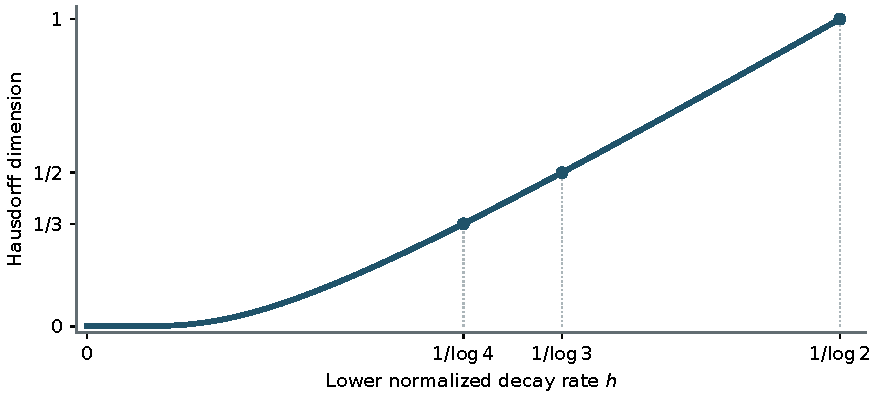
\includegraphics[width=0.82\linewidth]{spectrum.pdf}
\caption{Dimension of the set on which the lower decay rate equals $h$.
For instance, the rate $1/\log 3$ occurs on a set of dimension $1/2$.
The curve is the exact formula in Theorem~\ref{thm:dimension}.}
\end{figure}
\section{Two nearby peaks for the Riemann zeta function}
\label{sec:zetapeaks}
Write $a_j=2\arctan(1/(2\gamma_j))$ for the positive Cayley angle of the
$j$th positive zeta zero, indexed in increasing order of ordinate.
The first eight zeros are simple, so each $a_j$ with $1\le j\le8$ and its negative
carry unit jump intensity. The values used below come from
\href{https://www-users.cse.umn.edu/~odlyzko/zeta_tables/index.html}{Odlyzko's tables}.
The enclosed script \texttt{check\_zeta\_angles.py} propagates 24 decimal
places of the published ordinates using rational arithmetic and the
alternating series for $\arctan$. Completeness of the independently computed
Platt data is documented in the
\href{https://www.lmfdb.org/zeros/zeta/Source}{LMFDB source notes}.

On the line, the two largest distinct sums of $k$ jumps are $k a_1$
and $(k-1)a_1+a_2$. Both exceed the maximum $(k-1)a_1$ of all lower
orders. Attaining the first sum forces all $k$ jumps to equal $a_1$.
Attaining the second forces precisely one jump to equal $a_2$ and
all the others to equal $a_1$. Their local Cauchy coefficients are
therefore $1/k!$ and $1/(k-1)!$, respectively. The same proof applies
on the circle for $1\leq k\leq44$, since $44a_1<\pi$.
For $k=2$ these centers are approximately $0.14143652588586436844$ and
$0.11827841945959069544$.

A closer pair occurs at $u=2a_2$ and $v=a_1+a_7$. The rational enclosures give
\[
 0.00003542639447445315<v-u<0.00003542639447445316.
\]
Both are above $a_1$. Among two-jump sums with neither summand equal to
$a_1$, the largest is $2a_2$, achieved only by $(a_2,a_2)$.
Among sums using $a_1$, the consecutive angles $a_8$ and $a_7$ give
$a_1+a_8<u<v=a_1+a_7$. Hence $u$ and $v$ are consecutive two-jump
centers and their ordered representation counts are $1$ and $2$.
At either center the density has the same Cauchy profile on its shrinking
natural scale. The peak at $v$ is asymptotically twice as high as the
peak at $u$. These conclusions use the ordering of the full angle
sequence and allow arbitrary relations among the remaining ordinates.
\section{Further questions}
What are the dimensions of the joint level sets of the lower and upper
normalized decay rates? Section~\ref{sec:dimension} determines the marginal
level sets of the lower rate. Can the $O(L)$ loss in the uniform estimate
\eqref{eq:metriclower} be expanded further, and does any next term depend
on the conductor? Finally, what conductor-uniform separation estimates
for low-order Cayley sums can be proved for a restricted set of ordinates?
Such estimates would turn the finite-mode reading at the end of
Section~\ref{sec:finite} into a certified stopping rule.
\begin{thebibliography}{9}
\bibitem{lagarias} J. C. Lagarias, Li coefficients for automorphic
$L$-functions, \emph{Ann. Inst. Fourier} \textbf{57} (2007), 1689--1740.
\href{https://doi.org/10.5802/aif.2311}{doi:10.5802/aif.2311}.
\bibitem{nakamura} T. Nakamura and M. Suzuki, On infinitely divisible distributions
related to the Riemann hypothesis, \emph{Statist. Probab. Lett.} \textbf{201}
(2023), 109889. \href{https://doi.org/10.1016/j.spl.2023.109889}{doi:10.1016/j.spl.2023.109889}.
\bibitem{wu} J. Wu, On the distribution of denominators in Sylvester
expansions (II), \emph{Math. Proc. Cambridge Philos. Soc.} \textbf{135}
(2003), 421--430. \href{https://doi.org/10.1017/S0305004103006935}{doi:10.1017/S0305004103006935}.
\bibitem{picard1} J. Picard, Density in small time for L\'evy processes,
\emph{ESAIM Probab. Stat.} \textbf{1} (1997), 357--389.
\href{https://www.numdam.org/item/PS_1997__1__357_0/}{Article and full text}.
\bibitem{picard2} J. Picard, Density in small time at accessible points
for jump processes, \emph{Stochastic Process. Appl.} \textbf{67} (1997),
251--279. \href{https://lmbp.uca.fr/~picard/small_time.pdf}{Author's text}.
\end{thebibliography}
\end{document}
